% Requires graphicx; paths relative to the release root.
% Chinese captions need your thesis CJK/ctex setup.
\begin{figure}[htbp]
\centering
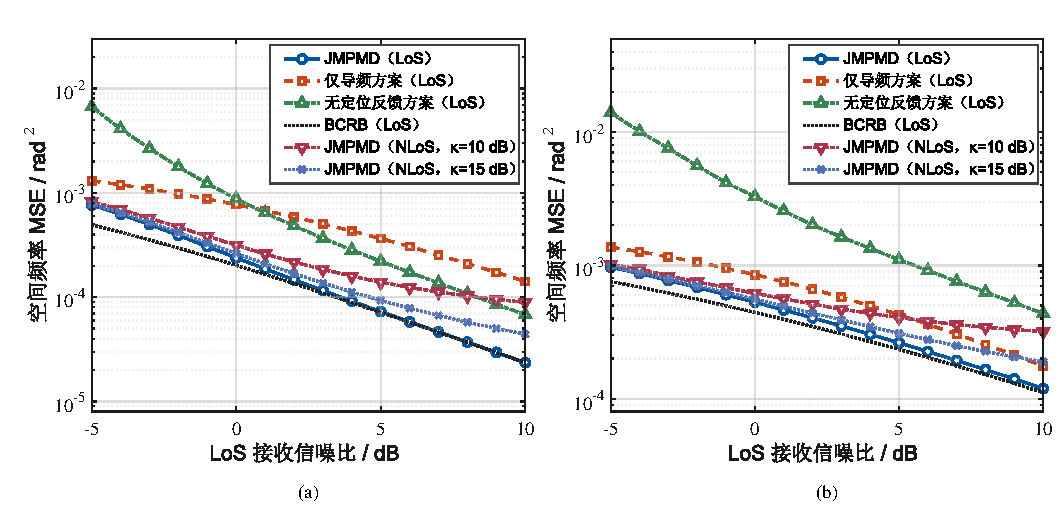
\includegraphics[width=\linewidth]{results/published/figures/thesis_A1_theta.pdf}
\caption{A1/A2：空间频率估计。（a）QPSK；（b）Gaussian。两者均采用严格矩和局部角度求峰；JMPMD 与无定位反馈方案首次系数用导频。A2 的 mixed20 NLoS JMPMD 曲线已并入；κ=10/15 dB，SNR 分子只含 LoS 功率。T=40、Tp=10；QPSK 7–10 dB 每点15000次，其余每点5000次。LoS 参考量不作为 NLoS 下界。BCRB 的信息假设沿用作者确认定义。}
\label{fig:thesis_A1_theta}
\end{figure}

\begin{figure}[htbp]
\centering
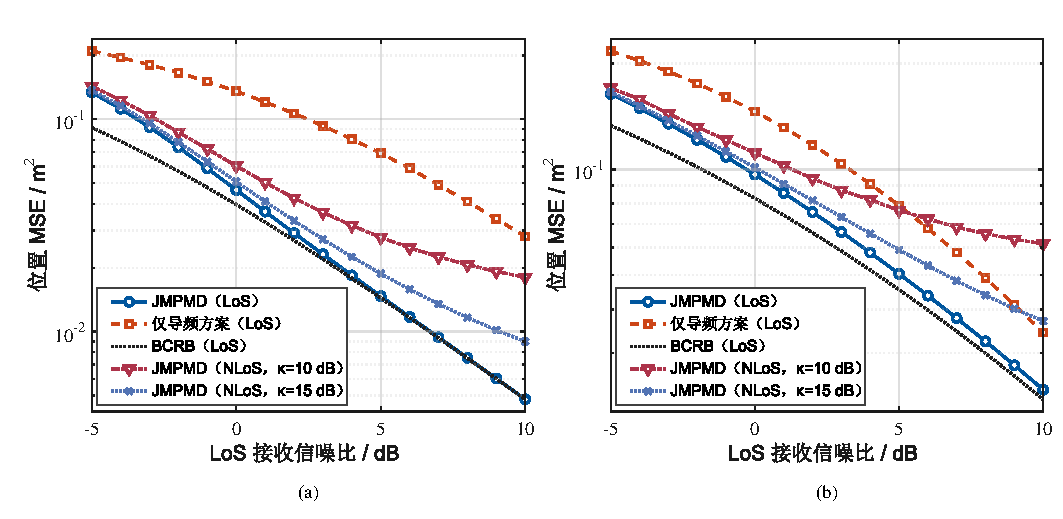
\includegraphics[width=\linewidth]{results/published/figures/thesis_A1_position.pdf}
\caption{A1/A2：用户定位。（a）QPSK；（b）Gaussian。两者均采用严格矩和局部角度求峰；JMPMD 与无定位反馈方案首次系数用导频。A2 的 mixed20 NLoS JMPMD 曲线已并入；κ=10/15 dB，SNR 分子只含 LoS 功率。T=40、Tp=10；QPSK 7–10 dB 每点15000次，其余每点5000次。LoS 参考量不作为 NLoS 下界。无定位反馈方案的最终一次定位放在补充图。}
\label{fig:thesis_A1_position}
\end{figure}

\begin{figure}[htbp]
\centering
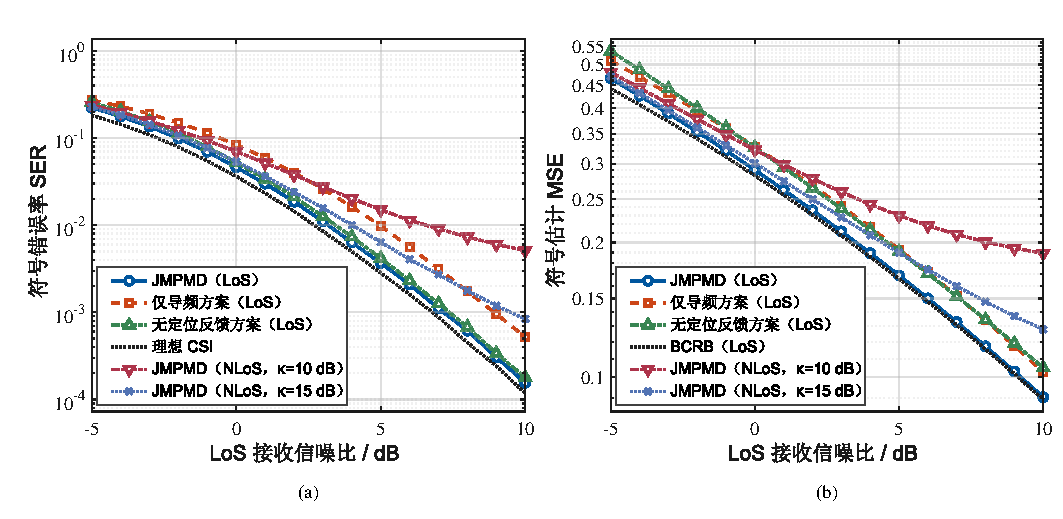
\includegraphics[width=\linewidth]{results/published/figures/thesis_A1_data.pdf}
\caption{A1/A2：数据检测。（a）QPSK；（b）Gaussian。两者均采用严格矩和局部角度求峰；JMPMD 与无定位反馈方案首次系数用导频。A2 的 mixed20 NLoS JMPMD 曲线已并入；κ=10/15 dB，SNR 分子只含 LoS 功率。T=40、Tp=10；QPSK 7–10 dB 每点15000次，其余每点5000次。LoS 参考量不作为 NLoS 下界。QPSK 为联合 MAP 的 SER，单条理想 CSI 基准使用完整噪声协方差；Gaussian 为后验均值 MSE，参考线为 BCRB。两种纵轴数值不可直接比较。}
\label{fig:thesis_A1_data}
\end{figure}

\begin{figure}[htbp]
\centering
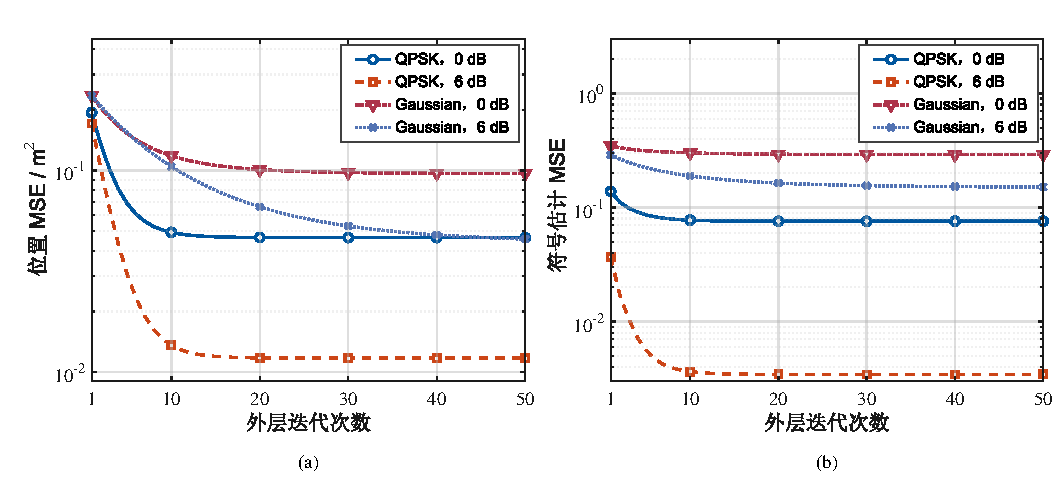
\includegraphics[width=\linewidth]{results/published/figures/thesis_A4_convergence.pdf}
\caption{A4：定位与符号检测的迭代性能。（a）位置 MSE；（b）符号估计 MSE。每子图为 QPSK/Gaussian × 0/6 dB 四条线。QPSK 使用离散后验均值的软符号误差；Gaussian 使用复符号后验均值误差，不将 SER 与 MSE 混画。每线5000条完整轨迹，早停后末值延拓。仅展示前50轮，实际外层上限仍为200；不据截取窗口宣称全部收敛。}
\label{fig:thesis_A4_convergence}
\end{figure}

\begin{figure}[htbp]
\centering
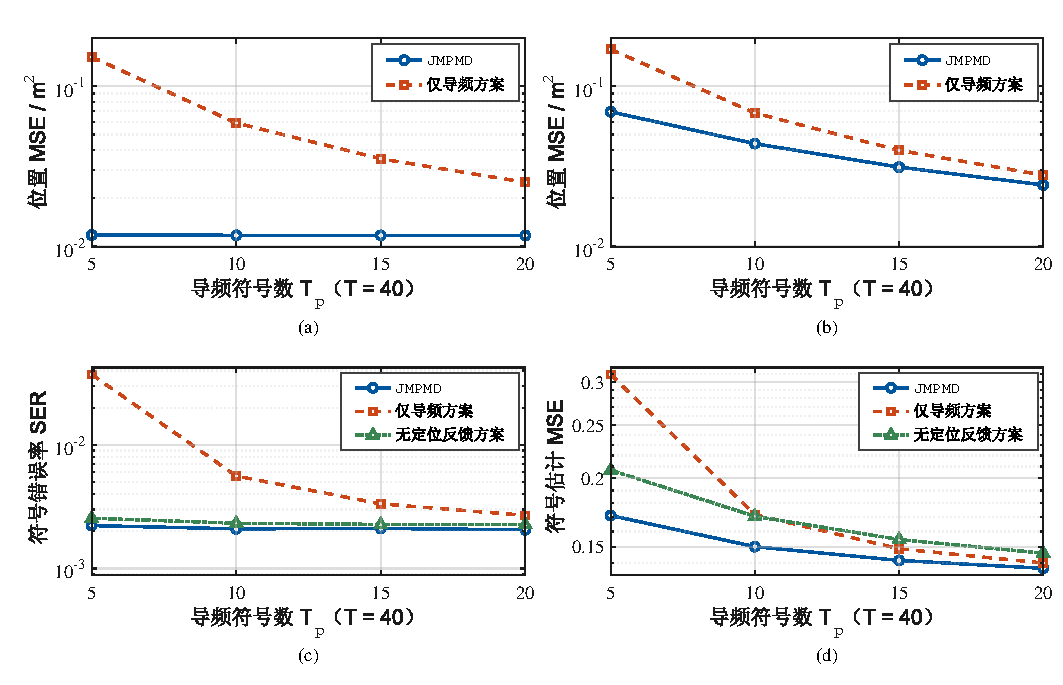
\includegraphics[width=\linewidth]{results/published/figures/thesis_B1_pilots.pdf}
\caption{B1：导频资源扫描。（a）QPSK 定位；（b）Gaussian 定位；（c）QPSK 检测；（d）Gaussian 检测。Q/G 均为严格矩、局部角度求峰，所有配置每点5000次。T=40，LoS SNR=6 dB。导频增多同时减少未知数据时隙，不能由单符号误差推断净吞吐量。}
\label{fig:thesis_B1_pilots}
\end{figure}

\begin{figure}[htbp]
\centering
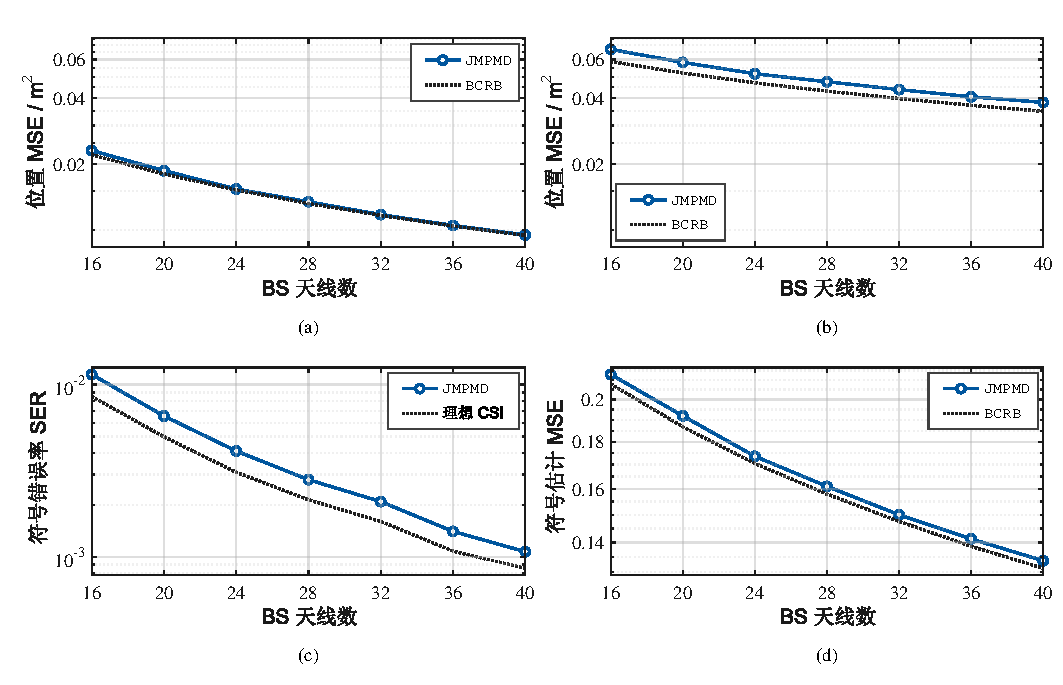
\includegraphics[width=\linewidth]{results/published/figures/thesis_A3_bs.pdf}
\caption{A3：BS 天线数扫描。（a）QPSK 定位；（b）Gaussian 定位；（c）QPSK 检测；（d）Gaussian 检测。Q/G 均为严格矩、局部角度求峰，所有配置每点5000次。LoS SNR=6 dB，保留位置先验角度初始化；未加 B3 的导频角度搜索。}
\label{fig:thesis_A3_bs}
\end{figure}

\begin{figure}[htbp]
\centering
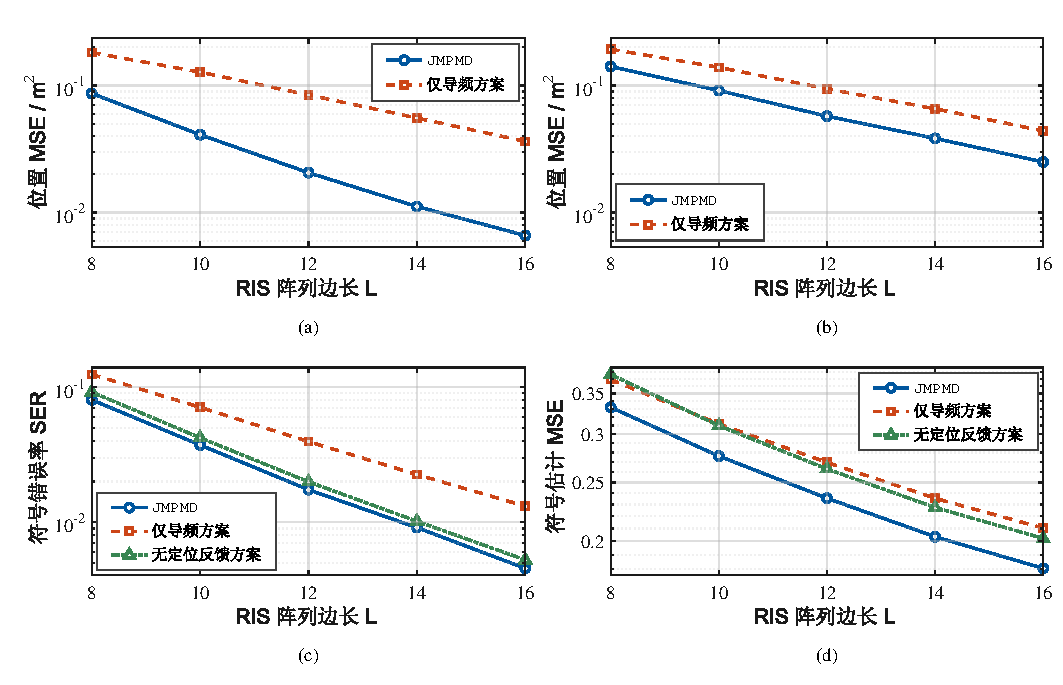
\includegraphics[width=\linewidth]{results/published/figures/thesis_B3_ris_size.pdf}
\caption{B3：RIS 边长扫描。（a）QPSK 定位；（b）Gaussian 定位；（c）QPSK 检测；（d）Gaussian 检测。Q/G 均为严格矩、局部角度求峰，所有配置每点5000次。L=8:2:16，Q/G 都使用先验约束导频角度初始化，首次系数同样用导频。固定发射功率25 dBm和噪声−125 dBm；接收 SNR 随阵列规模变化。本图不验证 L=20/24。}
\label{fig:thesis_B3_ris_size}
\end{figure}

